\chapter{Árboles de expansión}

\index{árbol de expansión}

Un \key{árbol de expansión} de un grafo consiste en
todos los nodos del grafo y algunas de las
aristas del grafo de modo que exista un camino
entre dos nodos cualesquiera.
Al igual que los árboles en general, los árboles de expansión son
conectados y acíclicos.
Por lo general, hay varias formas de construir un árbol de expansión.

Por ejemplo, considere el siguiente grafo:
\begin{center}
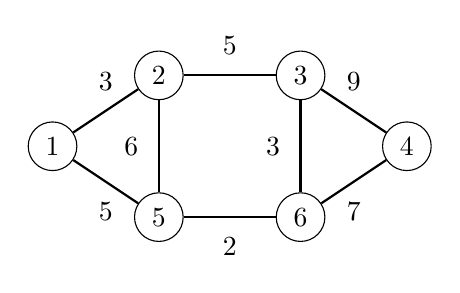
\begin{tikzpicture}[scale=0.9]
\node[draw, circle] (1) at (1.5,2) {$1$};
\node[draw, circle] (2) at (3,3) {$2$};
\node[draw, circle] (3) at (5,3) {$3$};
\node[draw, circle] (4) at (6.5,2) {$4$};
\node[draw, circle] (5) at (3,1) {$5$};
\node[draw, circle] (6) at (5,1) {$6$};
\path[draw,thick,-] (1) -- node[font=\small,label=above:3] {} (2);
\path[draw,thick,-] (2) -- node[font=\small,label=above:5] {} (3);
\path[draw,thick,-] (3) -- node[font=\small,label=above:9] {} (4);
\path[draw,thick,-] (1) -- node[font=\small,label=below:5] {} (5);
\path[draw,thick,-] (5) -- node[font=\small,label=below:2] {} (6);
\path[draw,thick,-] (6) -- node[font=\small,label=below:7] {} (4);
\path[draw,thick,-] (2) -- node[font=\small,label=left:6] {} (5);
\path[draw,thick,-] (3) -- node[font=\small,label=left:3] {} (6);
\end{tikzpicture}
\end{center}
Un árbol de expansión para el grafo es el siguiente:
\begin{center}
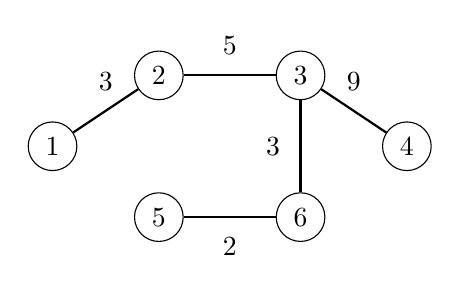
\begin{tikzpicture}[scale=0.9]
\node[draw, circle] (1) at (1.5,2) {$1$};
\node[draw, circle] (2) at (3,3) {$2$};
\node[draw, circle] (3) at (5,3) {$3$};
\node[draw, circle] (4) at (6.5,2) {$4$};
\node[draw, circle] (5) at (3,1) {$5$};
\node[draw, circle] (6) at (5,1) {$6$};
\path[draw,thick,-] (1) -- node[font=\small,label=above:3] {} (2);
\path[draw,thick,-] (2) -- node[font=\small,label=above:5] {} (3);
\path[draw,thick,-] (3) -- node[font=\small,label=above:9] {} (4);
\path[draw,thick,-] (5) -- node[font=\small,label=below:2] {} (6);
\path[draw,thick,-] (3) -- node[font=\small,label=left:3] {} (6);
\end{tikzpicture}
\end{center}

El peso de un árbol de expansión es la suma de los pesos de sus aristas.
Por ejemplo, el peso del árbol de expansión anterior es
$3+5+9+3+2=22$.

\index{árbol de expansión mínimo}

Un \key{árbol de expansión mínimo}
es un árbol de expansión cuyo peso es lo más pequeño posible.
El peso de un árbol de expansión mínimo para el grafo de ejemplo
es 20, y dicho árbol puede construirse de la siguiente manera:

\begin{center}
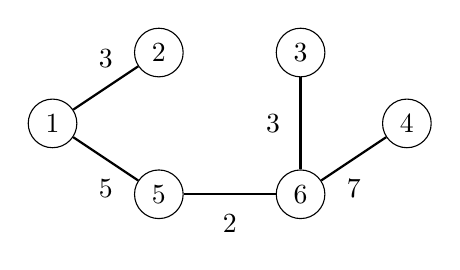
\begin{tikzpicture}[scale=0.9]
\node[draw, circle] (1) at (1.5,2) {$1$};
\node[draw, circle] (2) at (3,3) {$2$};
\node[draw, circle] (3) at (5,3) {$3$};
\node[draw, circle] (4) at (6.5,2) {$4$};
\node[draw, circle] (5) at (3,1) {$5$};
\node[draw, circle] (6) at (5,1) {$6$};

\path[draw,thick,-] (1) -- node[font=\small,label=above:3] {} (2);
\path[draw,thick,-] (1) -- node[font=\small,label=below:5] {} (5);
\path[draw,thick,-] (5) -- node[font=\small,label=below:2] {} (6);
\path[draw,thick,-] (6) -- node[font=\small,label=below:7] {} (4);
\path[draw,thick,-] (3) -- node[font=\small,label=left:3] {} (6);
\end{tikzpicture}
\end{center}

\index{árbol de expansión máximo}

De manera similar, un \key{árbol de expansión máximo}
es un árbol de expansión cuyo peso es lo más grande posible.
El peso de un árbol de expansión máximo para el
grafo de ejemplo es 32:

\begin{center}
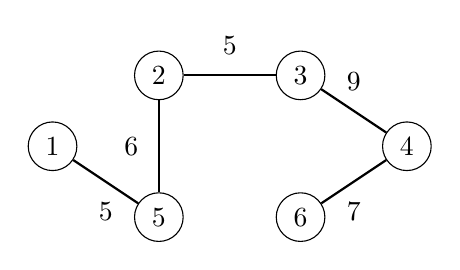
\begin{tikzpicture}[scale=0.9]
\node[draw, circle] (1) at (1.5,2) {$1$};
\node[draw, circle] (2) at (3,3) {$2$};
\node[draw, circle] (3) at (5,3) {$3$};
\node[draw, circle] (4) at (6.5,2) {$4$};
\node[draw, circle] (5) at (3,1) {$5$};
\node[draw, circle] (6) at (5,1) {$6$};
\path[draw,thick,-] (2) -- node[font=\small,label=above:5] {} (3);
\path[draw,thick,-] (3) -- node[font=\small,label=above:9] {} (4);
\path[draw,thick,-] (1) -- node[font=\small,label=below:5] {} (5);
\path[draw,thick,-] (6) -- node[font=\small,label=below:7] {} (4);
\path[draw,thick,-] (2) -- node[font=\small,label=left:6] {} (5);
\end{tikzpicture}
\end{center}

Tenga en cuenta que un grafo puede tener varios
árboles de expansión mínimos y máximos,
por lo que los árboles no son únicos.

Resulta que varios métodos voraces
se pueden utilizar para construir árboles de expansión mínimos y máximos.
En este capítulo, analizamos dos algoritmos
que procesan
las aristas del grafo ordenadas por sus pesos.
Nos centramos en encontrar árboles de expansión mínimos,
pero los mismos algoritmos pueden encontrar
árboles de expansión máximos procesando las aristas en orden inverso.

\section{Algoritmo de Kruskal}

\index{Algoritmo de Kruskal}

En el \key{algoritmo de Kruskal}\footnote{El algoritmo fue publicado en 1956
por J. B. Kruskal \cite{kru56}.}, el árbol de expansión inicial
solo contiene los nodos del grafo
y no contiene ninguna arista.
Luego, el algoritmo recorre las aristas
ordenado por sus pesos, y siempre agrega una arista
al árbol si no crea un ciclo.

El algoritmo mantiene los componentes
del árbol.
Inicialmente, cada nodo del grafo
pertenece a un componente separado.
Siempre que se agrega una arista al árbol,
se unen dos componentes.
Finalmente, todos los nodos pertenecen al mismo componente,
y se ha encontrado un árbol de expansión mínimo.

\subsubsection{Ejemplo}
\begin{samepage}
Consideremos cómo el algoritmo de Kruskal procesa el
siguiente gráfico:
\begin{center}
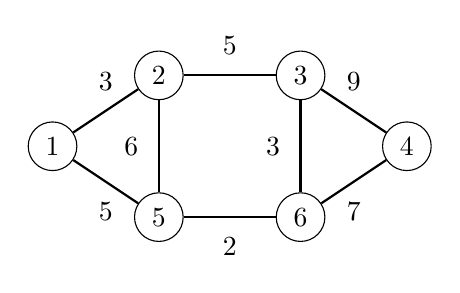
\begin{tikzpicture}[scale=0.9]
\node[draw, circle] (1) at (1.5,2) {$1$};
\node[draw, circle] (2) at (3,3) {$2$};
\node[draw, circle] (3) at (5,3) {$3$};
\node[draw, circle] (4) at (6.5,2) {$4$};
\node[draw, circle] (5) at (3,1) {$5$};
\node[draw, circle] (6) at (5,1) {$6$};
\path[draw,thick,-] (1) -- node[font=\small,label=above:3] {} (2);
\path[draw,thick,-] (2) -- node[font=\small,label=above:5] {} (3);
\path[draw,thick,-] (3) -- node[font=\small,label=above:9] {} (4);
\path[draw,thick,-] (1) -- node[font=\small,label=below:5] {} (5);
\path[draw,thick,-] (5) -- node[font=\small,label=below:2] {} (6);
\path[draw,thick,-] (6) -- node[font=\small,label=below:7] {} (4);
\path[draw,thick,-] (2) -- node[font=\small,label=left:6] {} (5);
\path[draw,thick,-] (3) -- node[font=\small,label=left:3] {} (6);
\end{tikzpicture}
\end{center}
\end{samepage}

\begin{samepage}
El primer paso del algoritmo es ordenar los
bordes en orden creciente de sus pesos.
El resultado es la siguiente lista:

\begin{tabular}{ll}
\\
borde & peso \\
\hline
5--6 & 2 \\
1--2 & 3 \\
3--6 & 3 \\
1--5 & 5 \\
2--3 & 5 \\
2--5 & 6 \\
4--6 & 7 \\
3--4 & 9 \\
\\
\end{tabular}
\end{samepage}

Después de esto, el algoritmo recorre la lista
y agrega cada borde al árbol si une
dos componentes separados.

Inicialmente, cada nodo está en su propio componente:

\begin{center}
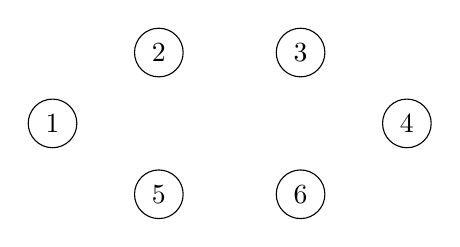
\begin{tikzpicture}[scale=0.9]
\node[draw, circle] (1) at (1.5,2) {$1$};
\node[draw, circle] (2) at (3,3) {$2$};
\node[draw, circle] (3) at (5,3) {$3$};
\node[draw, circle] (4) at (6.5,2) {$4$};
\node[draw, circle] (5) at (3,1) {$5$};
\node[draw, circle] (6) at (5,1) {$6$};
%\path[draw,thick,-] (1) -- node[font=\small,label=above:3] {} (2);
%\path[draw,thick,-] (2) -- node[font=\small,label=above:5] {} (3);
%\path[draw,thick,-] (3) -- node[font=\small,label=above:9] {} (4);
%\path[draw,thick,-] (1) -- node[font=\small,label=below:5] {} (5);
%\path[draw,thick,-] (5) -- node[font=\small,label=below:2] {} (6);
%\path[draw,thick,-] (6) -- node[font=\small,label=below:7] {} (4);
%\path[draw,thick,-] (2) -- node[font=\small,label=left:6] {} (5);
%\path[draw,thick,-] (3) -- node[font=\small,label=left:3] {} (6);
\end{tikzpicture}
\end{center}
El primer borde que se agregará al árbol es
el borde 5--6 que crea un componente $\{5,6\}$
al unir los componentes $\{5\}$ y $\{6\}$:

\begin{center}
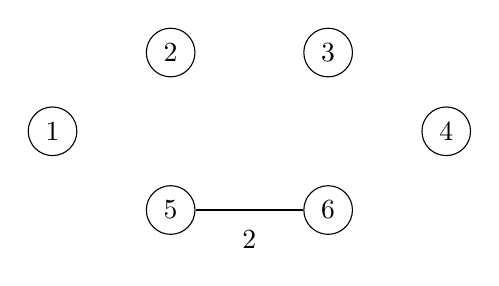
\begin{tikzpicture}
\node[draw, circle] (1) at (1.5,2) {$1$};
\node[draw, circle] (2) at (3,3) {$2$};
\node[draw, circle] (3) at (5,3) {$3$};
\node[draw, circle] (4) at (6.5,2) {$4$};
\node[draw, circle] (5) at (3,1) {$5$};
\node[draw, circle] (6) at (5,1) {$6$};

%\path[draw,thick,-] (1) -- node[font=\small,label=above:3] {} (2);
%\path[draw,thick,-] (2) -- node[font=\small,label=above:5] {} (3);
%\path[draw,thick,-] (3) -- node[font=\small,label=above:9] {} (4);
%\path[draw,thick,-] (1) -- node[font=\small,label=below:5] {} (5);
\path[draw,thick,-] (5) -- node[font=\small,label=below:2] {} (6);
%\path[draw,thick,-] (6) -- node[font=\small,label=below:7] {} (4);
%\path[draw,thick,-] (2) -- node[font=\small,label=left:6] {} (5);
%\path[draw,thick,-] (3) -- node[font=\small,label=left:3] {} (6);
\end{tikzpicture}
\end{center}
Después de esto, los bordes 1--2, 3--6 y 1--5 se agregan de manera similar:

\begin{center}
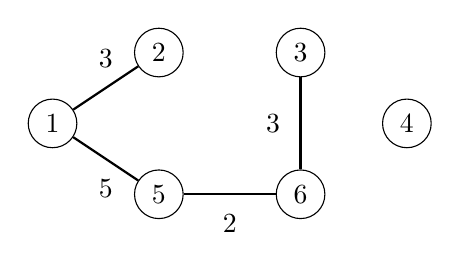
\begin{tikzpicture}[scale=0.9]
\node[draw, circle] (1) at (1.5,2) {$1$};
\node[draw, circle] (2) at (3,3) {$2$};
\node[draw, circle] (3) at (5,3) {$3$};
\node[draw, circle] (4) at (6.5,2) {$4$};
\node[draw, circle] (5) at (3,1) {$5$};
\node[draw, circle] (6) at (5,1) {$6$};

\path[draw,thick,-] (1) -- node[font=\small,label=above:3] {} (2);
%\path[draw,thick,-] (2) -- node[font=\small,label=above:5] {} (3);
%\path[draw,thick,-] (3) -- node[font=\small,label=above:9] {} (4);
\path[draw,thick,-] (1) -- node[font=\small,label=below:5] {} (5);
\path[draw,thick,-] (5) -- node[font=\small,label=below:2] {} (6);
%\path[draw,thick,-] (6) -- node[font=\small,label=below:7] {} (4);
%\path[draw,thick,-] (2) -- node[font=\small,label=left:6] {} (5);
\path[draw,thick,-] (3) -- node[font=\small,label=left:3] {} (6);
\end{tikzpicture}
\end{center}

Después de esos pasos, la mayoría de los componentes se han unido
y hay dos componentes en el árbol:
$\{1,2,3,5,6\}$ y $\{4\}$.

El siguiente borde en la lista es el borde 2--3,
pero no se incluirá en el árbol, porque
los nodos 2 y 3 ya están en el mismo componente.
Por la misma razón, el borde 2--5 no se incluirá en el árbol.

\begin{samepage}
Finalmente, el borde 4--6 se incluirá en el árbol:

\begin{center}
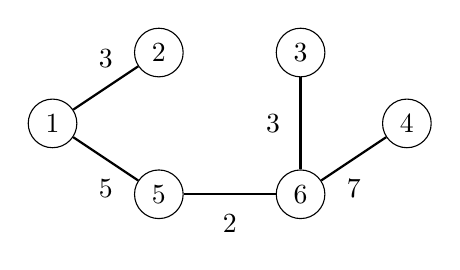
\begin{tikzpicture}[scale=0.9]
\node[draw, circle] (1) at (1.5,2) {$1$};
\node[draw, circle] (2) at (3,3) {$2$};
\node[draw, circle] (3) at (5,3) {$3$};
\node[draw, circle] (4) at (6.5,2) {$4$};
\node[draw, circle] (5) at (3,1) {$5$};
\node[draw, circle] (6) at (5,1) {$6$};

\path[draw,thick,-] (1) -- node[font=\small,label=above:3] {} (2);
%\path[draw,thick,-] (2) -- node[font=\small,label=above:5] {} (3);
%\path[draw,thick,-] (3) -- node[font=\small,label=above:9] {} (4);
\path[draw,thick,-] (1) -- node[font=\small,label=below:5] {} (5);
\path[draw,thick,-] (5) -- node[font=\small,label=below:2] {} (6);
\path[draw,thick,-] (6) -- node[font=\small,label=below:7] {} (4);
%\path[draw,thick,-] (2) -- node[font=\small,label=left:6] {} (5);
\path[draw,thick,-] (3) -- node[font=\small,label=left:3] {} (6);
\end{tikzpicture}
\end{center}
\end{samepage}

Después de esto, el algoritmo no agregará ningún
borde nuevo, porque el gráfico está conectado
y hay una ruta entre dos nodos.
El gráfico resultante es un árbol de expansión mínimo
con peso $2+3+3+5+7=20$.

\subsubsection{¿Por qué funciona esto?}

Es una buena pregunta por qué funciona el algoritmo de Kruskal.
¿Por qué la estrategia codiciosa garantiza que nosotros
encontrar un árbol de expansión mínimo?

Veamos qué pasa si el borde de peso mínimo de
el gráfico \emph{no} está incluido en el árbol de expansión.
Por ejemplo, supongamos que un árbol de expansión
para el gráfico anterior no contendría el
borde de peso mínimo 5--6.
No sabemos la estructura exacta de tal árbol de expansión,
pero en cualquier caso tiene que contener algunos bordes.
Asuma que el árbol sería como sigue:

\begin{center}
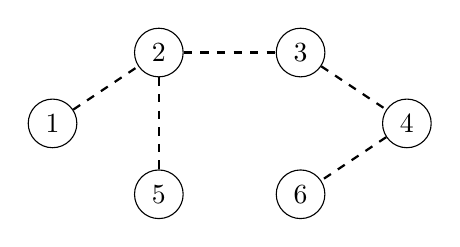
\begin{tikzpicture}[scale=0.9]
\node[draw, circle] (1) at (1.5,2) {$1$};
\node[draw, circle] (2) at (3,3) {$2$};
\node[draw, circle] (3) at (5,3) {$3$};
\node[draw, circle] (4) at (6.5,2) {$4$};
\node[draw, circle] (5) at (3,1) {$5$};
\node[draw, circle] (6) at (5,1) {$6$};

\path[draw,thick,-,dashed] (1) -- (2);
\path[draw,thick,-,dashed] (2) -- (5);
\path[draw,thick,-,dashed] (2) -- (3);
\path[draw,thick,-,dashed] (3) -- (4);
\path[draw,thick,-,dashed] (4) -- (6);
\end{tikzpicture}
\end{center}

Sin embargo, no es posible que el árbol anterior
sería un árbol de expansión mínimo para el gráfico.
La razón de esto es que podemos eliminar un borde
del árbol y reemplazarlo con el borde de peso mínimo 5--6.
Esto produce un árbol de expansión cuyo peso es
\emph{más pequeño}:

\begin{center}
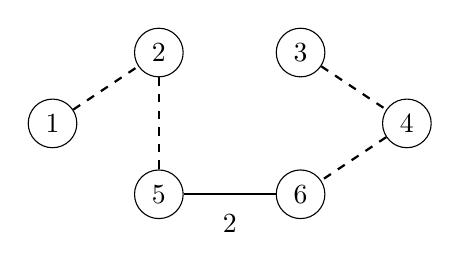
\begin{tikzpicture}[scale=0.9]
\node[draw, circle] (1) at (1.5,2) {$1$};
\node[draw, circle] (2) at (3,3) {$2$};
\node[draw, circle] (3) at (5,3) {$3$};
\node[draw, circle] (4) at (6.5,2) {$4$};
\node[draw, circle] (5) at (3,1) {$5$};
\node[draw, circle] (6) at (5,1) {$6$};

\path[draw,thick,-,dashed] (1) -- (2);
\path[draw,thick,-,dashed] (2) -- (5);
\path[draw,thick,-,dashed] (3) -- (4);
\path[draw,thick,-,dashed] (4) -- (6);
\path[draw,thick,-] (5) -- node[font=\small,label=below:2] {} (6);
\end{tikzpicture}
\end{center}

Por esta razón, siempre es óptimo
incluir el borde de peso mínimo
en el árbol para producir un árbol de expansión mínimo.
Usando un argumento similar, podemos mostrar que es
también es óptimo agregar el siguiente borde en orden de peso
al árbol, y así sucesivamente.
Por lo tanto, el algoritmo de Kruskal funciona correctamente y
siempre produce un árbol de expansión mínimo.

\subsubsection{Implementación}

Al implementar el algoritmo de Kruskal,
es conveniente usar
la representación de la lista de bordes del gráfico.
La primera fase del algoritmo ordena la
bordes en la lista en $O(m \log m)$ tiempo.
Después de esto, la segunda fase del algoritmo
construye el árbol de expansión mínimo como sigue:

\begin{lstlisting}
for (...) {
  if (!same(a,b)) unite(a,b);
}
\end{lstlisting}

El bucle recorre los bordes de la lista
y siempre procesa un borde $a$--$b$
donde $a$ y $b$ son dos nodos.
Se necesitan dos funciones:
la función \texttt{same} determina
si $a$ y $b$ están en el mismo componente,
y la función \texttt{unite}
une los componentes que contienen $a$ y $b$.

El problema es cómo implementar eficientemente
las funciones \texttt{same} y \texttt{unite}.
Una posibilidad es implementar la función
\texttt{same} como un recorrido del gráfico y verificar si
podemos obtener del nodo $a$ al nodo $b$.
Sin embargo, la complejidad temporal de tal función
sería $O(n+m)$
y el algoritmo resultante sería lento,
porque la función \texttt{same} se llamará para cada borde del gráfico.

Resolveremos el problema utilizando una estructura de unión-búsqueda
que implementa ambas funciones en $O(\log n)$ tiempo.
Por lo tanto, la complejidad temporal del algoritmo de Kruskal
será $O(m \log n)$ después de ordenar la lista de bordes.

\section{Estructura de unión-búsqueda}

\index{estructura de unión-búsqueda}

Una \key{estructura de unión-búsqueda} mantiene
una colección de conjuntos.
Los conjuntos son disjuntos, por lo que ningún elemento
pertenece a más de un conjunto.
Se admiten dos operaciones de tiempo $O(\log n)$:
la operación \texttt{unite} une dos conjuntos,
y la operación \texttt{find} encuentra el representante
del conjunto que contiene un elemento dado\footnote{La estructura presentada aquí
fue introducida en 1971 por J. D. Hopcroft y J. D. Ullman \cite{hop71}.
Más tarde, en 1975, R. E. Tarjan estudió una variante más sofisticada
de la estructura \cite{tar75} que se discute en muchos algoritmos
libros de texto hoy en día.}.

\subsubsection{Estructura}
En una estructura de unión-búsqueda, un elemento en cada conjunto
es el representante del conjunto,
y hay una cadena desde cualquier otro elemento del
conjunto hasta el representante.
Por ejemplo, suponga que los conjuntos son
$\{1,4,7\}$, $\{5\}$ y $\{2,3,6,8\}$:
\begin{center}
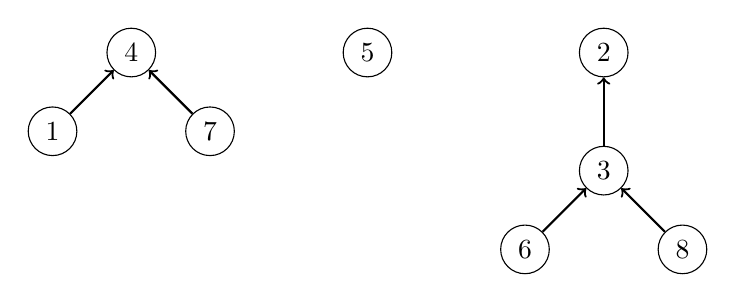
\begin{tikzpicture}
\node[draw, circle] (1) at (0,-1) {$1$};
\node[draw, circle] (2) at (7,0) {$2$};
\node[draw, circle] (3) at (7,-1.5) {$3$};
\node[draw, circle] (4) at (1,0) {$4$};
\node[draw, circle] (5) at (4,0) {$5$};
\node[draw, circle] (6) at (6,-2.5) {$6$};
\node[draw, circle] (7) at (2,-1) {$7$};
\node[draw, circle] (8) at (8,-2.5) {$8$};

\path[draw,thick,->] (1) -- (4);
\path[draw,thick,->] (7) -- (4);

\path[draw,thick,->] (3) -- (2);
\path[draw,thick,->] (6) -- (3);
\path[draw,thick,->] (8) -- (3);

\end{tikzpicture}
\end{center}
En este caso, los representantes
de los conjuntos son 4, 5 y 2.
Podemos encontrar el representante de cualquier elemento
siguiendo la cadena que comienza en el elemento.
Por ejemplo, el elemento 2 es el representante
para el elemento 6, porque
seguimos la cadena $6 \rightarrow 3 \rightarrow 2$.
Dos elementos pertenecen al mismo conjunto exactamente cuando
sus representantes son los mismos.

Dos conjuntos se pueden unir conectando el
representante de un conjunto al
representante del otro conjunto.
Por ejemplo, los conjuntos
$\{1,4,7\}$ y $\{2,3,6,8\}$
se pueden unir de la siguiente manera:
\begin{center}
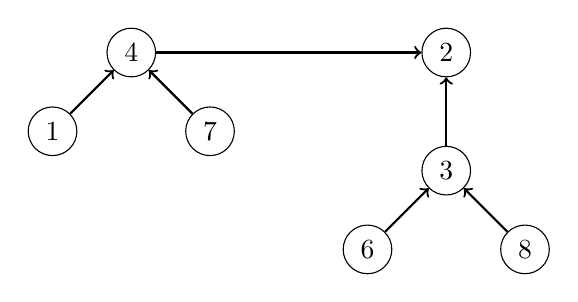
\begin{tikzpicture}
\node[draw, circle] (1) at (2,-1) {$1$};
\node[draw, circle] (2) at (7,0) {$2$};
\node[draw, circle] (3) at (7,-1.5) {$3$};
\node[draw, circle] (4) at (3,0) {$4$};
\node[draw, circle] (6) at (6,-2.5) {$6$};
\node[draw, circle] (7) at (4,-1) {$7$};
\node[draw, circle] (8) at (8,-2.5) {$8$};

\path[draw,thick,->] (1) -- (4);
\path[draw,thick,->] (7) -- (4);

\path[draw,thick,->] (3) -- (2);
\path[draw,thick,->] (6) -- (3);
\path[draw,thick,->] (8) -- (3);

\path[draw,thick,->] (4) -- (2);
\end{tikzpicture}
\end{center}

El conjunto resultante contiene los elementos
$\{1,2,3,4,6,7,8\}$.
A partir de este momento, el elemento 2 es el representante
de todo el conjunto y el antiguo representante 4
apunta al elemento 2.

La eficiencia de la estructura de unión-búsqueda depende de
cómo se unen los conjuntos.
Resulta que podemos seguir una estrategia simple:
siempre conectar el representante del
conjunto \emph{más pequeño} al representante del conjunto \emph{más grande}
(o si los conjuntos son del mismo tamaño,
podemos hacer una elección arbitraria).
Usando esta estrategia, la longitud de cualquier cadena
será $O(\log n)$, por lo que podemos
encontrar el representante de cualquier elemento
eficientemente siguiendo la cadena correspondiente.

\subsubsection{Implementación}

La estructura de unión-búsqueda se puede implementar
usando matrices.
En la siguiente implementación,
la matriz \texttt{link} contiene para cada elemento
el siguiente elemento
en la cadena o el elemento mismo si es
un representante,
y la matriz \texttt{size} indica para cada representante
el tamaño del conjunto correspondiente.

Inicialmente, cada elemento pertenece a un conjunto separado:
\begin{lstlisting}
for (int i = 1; i <= n; i++) link[i] = i;
for (int i = 1; i <= n; i++) size[i] = 1;
\end{lstlisting}

La función \texttt{find} devuelve
el representante para un elemento $x$.
El representante se puede encontrar siguiendo
la cadena que comienza en $x$.

\begin{lstlisting}
int find(int x) {
    while (x != link[x]) x = link[x];
    return x;
}
\end{lstlisting}

La función \texttt{same} comprueba
si los elementos $a$ y $b$ pertenecen al mismo conjunto.
Esto se puede hacer fácilmente utilizando el
función \texttt{find}:

\begin{lstlisting}
bool same(int a, int b) {
    return find(a) == find(b);
}
\end{lstlisting}

\begin{samepage}
La función \texttt{unite} une los conjuntos
que contienen los elementos $a$ y $b$
(los elementos deben estar en conjuntos diferentes).
La función primero encuentra los representantes
de los conjuntos y luego conecta el más pequeño
conjunto al conjunto más grande.

\begin{lstlisting}
void unite(int a, int b) {
    a = find(a);
    b = find(b);
    if (size[a] < size[b]) swap(a,b);
    size[a] += size[b];
    link[b] = a;
}
\end{lstlisting}
\end{samepage}

La complejidad temporal de la función \texttt{find}
es $O(\log n)$ asumiendo que la longitud de cada
cadena es $O(\log n)$.
En este caso, las funciones \texttt{same} y \texttt{unite}
también funcionan en tiempo $O(\log n)$.
La función \texttt{unite} se asegura de que el
longitud de cada cadena es $O(\log n)$ conectando
el conjunto más pequeño al conjunto más grande.

\section{Algoritmo de Prim}

\index{Algoritmo de Prim}

\key{Algoritmo de Prim}\footnote{El algoritmo es
nombrado después de R. C. Prim quien lo publicó en 1957 \cite{pri57}.
Sin embargo, el mismo algoritmo ya fue descubierto en 1930
por V. Jarník.} es un método alternativo
para encontrar un árbol de expansión mínimo.
El algoritmo primero agrega un nodo arbitrario
al árbol.
Después de esto, el algoritmo siempre elige
un borde de peso mínimo que
agrega un nuevo nodo al árbol.
Finalmente, todos los nodos han sido agregados al árbol
y se ha encontrado un árbol de expansión mínimo.



El algoritmo de Prim se parece al algoritmo de Dijkstra.
La diferencia es que el algoritmo de Dijkstra siempre
selecciona una arista cuya distancia desde el nodo de inicio
es mínima, pero el algoritmo de Prim simplemente selecciona
la arista de peso mínimo que agrega un nuevo nodo al árbol.

\subsubsection{Ejemplo}

Consideremos cómo funciona el algoritmo de Prim
en el siguiente gráfico:

\begin{center}
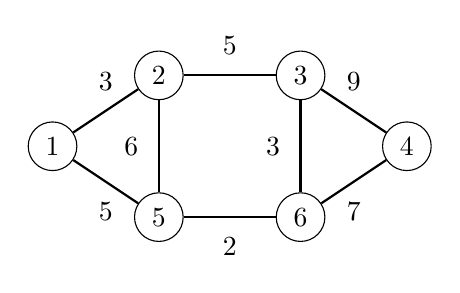
\begin{tikzpicture}[scale=0.9]
\node[draw, circle] (1) at (1.5,2) {$1$};
\node[draw, circle] (2) at (3,3) {$2$};
\node[draw, circle] (3) at (5,3) {$3$};
\node[draw, circle] (4) at (6.5,2) {$4$};
\node[draw, circle] (5) at (3,1) {$5$};
\node[draw, circle] (6) at (5,1) {$6$};
\path[draw,thick,-] (1) -- node[font=\small,label=above:3] {} (2);
\path[draw,thick,-] (2) -- node[font=\small,label=above:5] {} (3);
\path[draw,thick,-] (3) -- node[font=\small,label=above:9] {} (4);
\path[draw,thick,-] (1) -- node[font=\small,label=below:5] {} (5);
\path[draw,thick,-] (5) -- node[font=\small,label=below:2] {} (6);
\path[draw,thick,-] (6) -- node[font=\small,label=below:7] {} (4);
\path[draw,thick,-] (2) -- node[font=\small,label=left:6] {} (5);
\path[draw,thick,-] (3) -- node[font=\small,label=left:3] {} (6);

%\path[draw=red,thick,-,line width=2pt] (5) -- (6);
\end{tikzpicture}
\end{center}
Inicialmente, no hay aristas entre los nodos:
\begin{center}
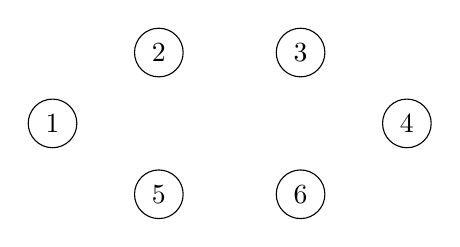
\begin{tikzpicture}[scale=0.9]
\node[draw, circle] (1) at (1.5,2) {$1$};
\node[draw, circle] (2) at (3,3) {$2$};
\node[draw, circle] (3) at (5,3) {$3$};
\node[draw, circle] (4) at (6.5,2) {$4$};
\node[draw, circle] (5) at (3,1) {$5$};
\node[draw, circle] (6) at (5,1) {$6$};
%\path[draw,thick,-] (1) -- node[font=\small,label=above:3] {} (2);
%\path[draw,thick,-] (2) -- node[font=\small,label=above:5] {} (3);
%\path[draw,thick,-] (3) -- node[font=\small,label=above:9] {} (4);
%\path[draw,thick,-] (1) -- node[font=\small,label=below:5] {} (5);
%\path[draw,thick,-] (5) -- node[font=\small,label=below:2] {} (6);
%\path[draw,thick,-] (6) -- node[font=\small,label=below:7] {} (4);
%\path[draw,thick,-] (2) -- node[font=\small,label=left:6] {} (5);
%\path[draw,thick,-] (3) -- node[font=\small,label=left:3] {} (6);
\end{tikzpicture}
\end{center}
Un nodo arbitrario puede ser el nodo de inicio,
así que elijamos el nodo 1.
Primero, agregamos el nodo 2 que está conectado por
una arista de peso 3:
\begin{center}
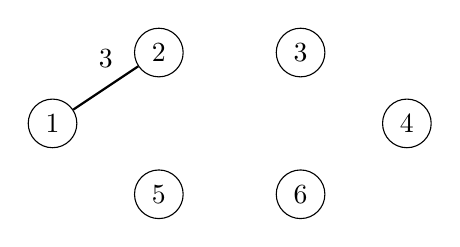
\begin{tikzpicture}[scale=0.9]
\node[draw, circle] (1) at (1.5,2) {$1$};
\node[draw, circle] (2) at (3,3) {$2$};
\node[draw, circle] (3) at (5,3) {$3$};
\node[draw, circle] (4) at (6.5,2) {$4$};
\node[draw, circle] (5) at (3,1) {$5$};
\node[draw, circle] (6) at (5,1) {$6$};
\path[draw,thick,-] (1) -- node[font=\small,label=above:3] {} (2);
%\path[draw,thick,-] (2) -- node[font=\small,label=above:5] {} (3);
%\path[draw,thick,-] (3) -- node[font=\small,label=above:9] {} (4);
%\path[draw,thick,-] (1) -- node[font=\small,label=below:5] {} (5);
%\path[draw,thick,-] (5) -- node[font=\small,label=below:2] {} (6);
%\path[draw,thick,-] (6) -- node[font=\small,label=below:7] {} (4);
%\path[draw,thick,-] (2) -- node[font=\small,label=left:6] {} (5);
%\path[draw,thick,-] (3) -- node[font=\small,label=left:3] {} (6);
\end{tikzpicture}
\end{center}

Después de esto, hay dos aristas con peso 5,
por lo que podemos agregar el nodo 3 o el nodo 5 al árbol.
Agreguemos el nodo 3 primero:
\begin{center}
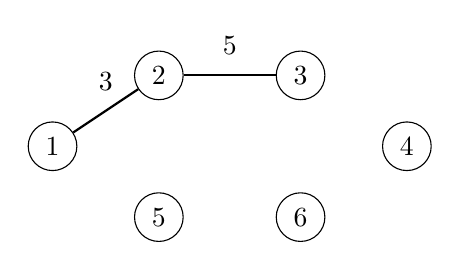
\begin{tikzpicture}[scale=0.9]
\node[draw, circle] (1) at (1.5,2) {$1$};
\node[draw, circle] (2) at (3,3) {$2$};
\node[draw, circle] (3) at (5,3) {$3$};
\node[draw, circle] (4) at (6.5,2) {$4$};
\node[draw, circle] (5) at (3,1) {$5$};
\node[draw, circle] (6) at (5,1) {$6$};
\path[draw,thick,-] (1) -- node[font=\small,label=above:3] {} (2);
\path[draw,thick,-] (2) -- node[font=\small,label=above:5] {} (3);
%\path[draw,thick,-] (3) -- node[font=\small,label=above:9] {} (4);
%\path[draw,thick,-] (1) -- node[font=\small,label=below:5] {} (5);
%\path[draw,thick,-] (5) -- node[font=\small,label=below:2] {} (6);
%\path[draw,thick,-] (6) -- node[font=\small,label=below:7] {} (4);
%\path[draw,thick,-] (2) -- node[font=\small,label=left:6] {} (5);
%\path[draw,thick,-] (3) -- node[font=\small,label=left:3] {} (6);
\end{tikzpicture}
\end{center}



\begin{samepage}
El proceso continúa hasta que todos los nodos se han incluido en el árbol:
\begin{center}
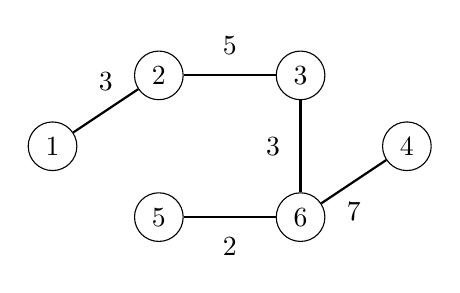
\begin{tikzpicture}[scale=0.9]
\node[draw, circle] (1) at (1.5,2) {$1$};
\node[draw, circle] (2) at (3,3) {$2$};
\node[draw, circle] (3) at (5,3) {$3$};
\node[draw, circle] (4) at (6.5,2) {$4$};
\node[draw, circle] (5) at (3,1) {$5$};
\node[draw, circle] (6) at (5,1) {$6$};
\path[draw,thick,-] (1) -- node[font=\small,label=above:3] {} (2);
\path[draw,thick,-] (2) -- node[font=\small,label=above:5] {} (3);
%\path[draw,thick,-] (3) -- node[font=\small,label=above:9] {} (4);
%\path[draw,thick,-] (1) -- node[font=\small,label=below:5] {} (5);
\path[draw,thick,-] (5) -- node[font=\small,label=below:2] {} (6);
\path[draw,thick,-] (6) -- node[font=\small,label=below:7] {} (4);
%\path[draw,thick,-] (2) -- node[font=\small,label=left:6] {} (5);
\path[draw,thick,-] (3) -- node[font=\small,label=left:3] {} (6);
\end{tikzpicture}
\end{center}
\end{samepage}

\subsubsection{Implementación}

Al igual que el algoritmo de Dijkstra, el algoritmo de Prim se puede
implementar de manera eficiente utilizando una cola de prioridad.
La cola de prioridad debe contener todos los nodos
que se pueden conectar al componente actual utilizando
un solo borde, en orden creciente de los pesos
de los bordes correspondientes.

La complejidad temporal del algoritmo de Prim es
$O(n + m \log m)$ que es igual a la complejidad temporal
del algoritmo de Dijkstra.
En la práctica, los algoritmos de Prim y Kruskal
son ambos eficientes, y la elección del algoritmo
es una cuestión de gusto.
Aún así, la mayoría de los programadores competitivos utilizan el algoritmo de Kruskal. 
